\chapter{Calibration}

In order to achieve high fidelity imaging, any systematic offsets of the radar sensor must be compensated.
In this chapter, the systematic errors of the radar are observed and classified (sec. \ref{sec:stability_analysis}). With knowledge of their stability and overall characteristics,
an online calibration method is implemented and its performance analised (sec. \ref{sec:calibration}).


\section{Stability Analysis}
\label{sec:stability_analysis}
The systematic errors described in section <> manifest by distorting amplitude and phase of each channel's deramped signal.
Static calibration is feasible if the systematic errors are not affected by changes of the following variables:
system restart, time elapsed since system restart, system temperature and the deramped signal's frequency.


\subsection{Setup}
The sensor is placed in a low-reflection environment and a corner reflector is placed at boresight in front of the sensor at a distance of roughly \SI{1.60}{\m} (cf. \ref{fig:photo_setup}).
The time data collected in all channels is recorded every minute.
The temperature readings of the sensor's CPU, FPGA and radar frontend are also recorded every minute (cf. \ref{fig:act_temp}).
The experiment is repeated with a different ramp slope $\dot \omega$ in order to achieve a different frequency of the deramped signal, since
\begin{align}
    f_{IF} = \dot \omega \cdot \frac{2 r_{refl}}{c}
\end{align}
\begin{figure}
    \centering
    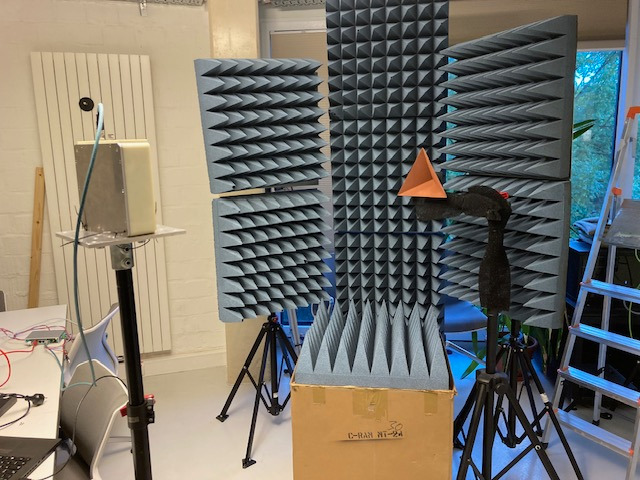
\includegraphics[height=0.25\textheight]{../figures/aufbau1.jpg}
    \caption{Measurement Setup}
    \label{fig:photo_setup}
\end{figure}
\begin{figure}
    \centering
    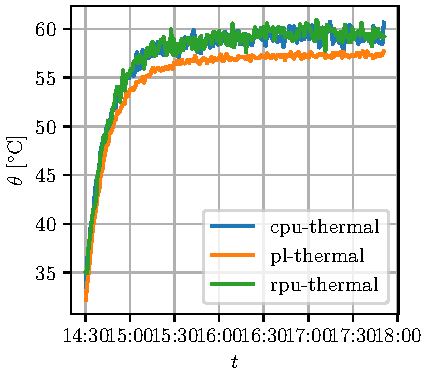
\includegraphics[height=0.25\textheight]{../figures/actual_temperature.pdf}
    \caption{Measured System Temperature After Startup}
    \label{fig:act_temp}
\end{figure}

Due to the geometry of the setup, the runtime of each transmitted wavefront should be identical.
Thus, the ideal deramped signal should be of a single, constant frequency and without inter-channel phase differences.
\begin{figure}
    \centering
    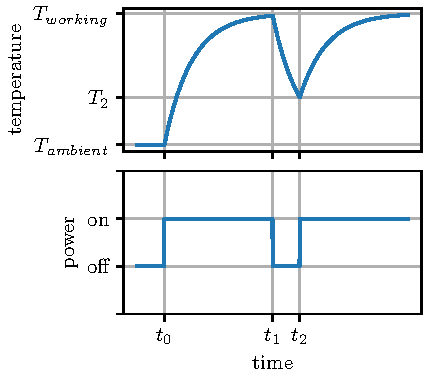
\includegraphics[height=0.25\textheight]{../figures/expected_temperature.pdf}
    \caption{Expected System Temperature over Time for Interrupted Power}
    \label{fig:exp_temp}
\end{figure}
In practice, the reflector peak will have a certain bandwidth,
and other peaks at higher and lower frequencies will be present due to incomplete shielding and/or unwanted reflections.
Also, the reflector peak may wander if the setup geometry moves. \\
For analysis, system runtime and temperature cannot be considered independent variables, as illustrated in figure \ref{fig:exp_temp}:
The system starts at ambient temperature, heating up and approaching a stable operating temperature on turning on ($t_0$), and cooling back down after turning off ($t_1$). \\
\subsection{Results}
\begin{figure}[h]
    \centering
    \begin{subfigure}[t]{.45\textwidth}
        \centering
        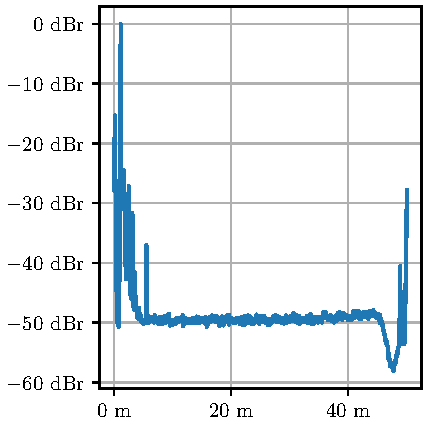
\includegraphics[width=\textwidth]{../figures/interference.pdf}
        \caption{Complete Spectrum}
    \end{subfigure}
    \begin{subfigure}[t]{.45\textwidth}
        \centering
        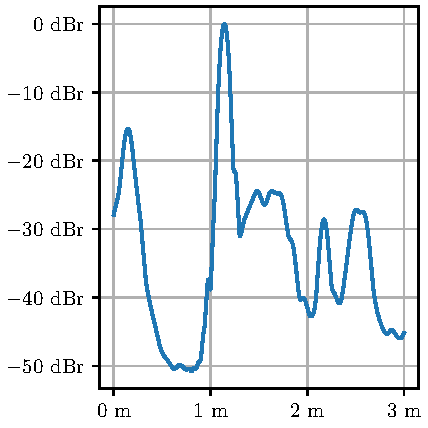
\includegraphics[width=\textwidth]{../figures/interference_zoom.pdf}
        \caption{Zoomed in}
    \end{subfigure}
    \caption{Mean Intensity Spectrum}
    \label{fig:avg_intensity}
\end{figure}
\subsubsection*{Preprocessing and Analysis}
Because of the aforementioned imperfections in the experiment, some preprocessing is required to analize the systematic offsets present in the radar signal.
Multiple additional peaks in the spectrum are visible in figure \ref{fig:avg_intensity}; indeed, the maximum peak is not even caused by the reflector.
It is therefore necessary to limit the analysis to only the FFT-bin at the maximum of the peak caused by the reflector.

The measurement environment also exhibits some minor changes in temperature and humidity, which can result in the geometry to shift by a few millimeters.
This shows by the spectral maximum shifting over time, as seen in figure \ref{fig:refldist}.

\begin{figure}
    \centering
    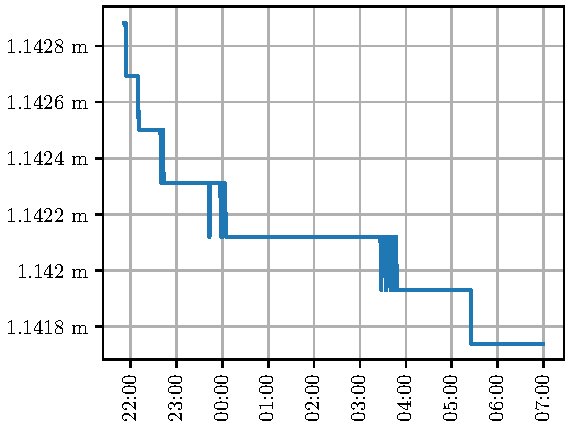
\includegraphics[height=0.25\textheight]{../figures/refldist.pdf}
    \caption{Change in reflector distance as measured by iMCR}
    \label{fig:refldist}
\end{figure}

In the following analysis, the main metric is the complex ratio of the maximum FFT-bin to its initial value.
Using a logarithmic representation  of this ratio, it can be represented as a level difference [\unit{\decibel}] and a phase difference [\unit{\degree}].

\subsubsection*{Effects of System Temperature and Runtime}

Multiple measurements have indicated that, while the amplitude rarely varies by more than \SI{1}{\decibel}, the phase is not as stable over time.
Typically, the mean phase drifts by up to \SI{50}{\degree} in the hours after system startup, with the rate of change reducing after around four hours.
However, it has to be noted that there is no clear correlation between phase drift and temperature:
the phase continues to drift after the system temperature stabilizes;
the reduction in drift only occurs hours after the system has reached a stable temperature of approximately \SI{60}{\celsius}.

\begin{figure}
    \centering
    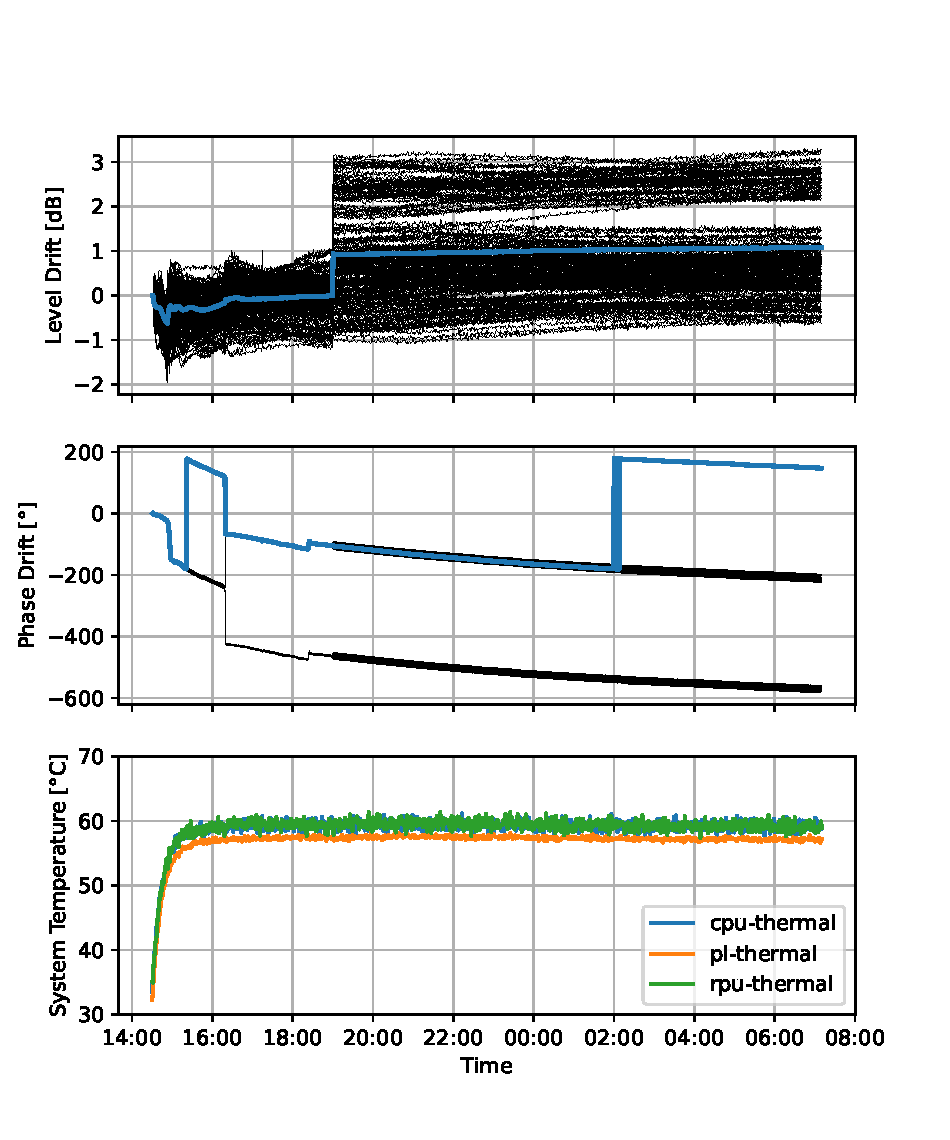
\includegraphics[width=\textwidth]{../figures/meas_23-10-09_phase_drift.pdf}
    \caption{Recorded drift over night}
    \label{fig:weekend}
\end{figure}

\subsubsection*{Effects of Self-Calibration}
As described in the specification, the AWR2243P-chips undergo a self-calibration upon initialization.
This initialization can be triggered by either restarting the entire system or by re-writing the configuration registers on the radar chips.
Indeed, this initial calibration can be observed in the data (cf. \ref{fig:restart}). After the connection with the radar has been re-established, the following effects are visible:
\begin{itemize}
    \item slightly increased level: the level in each channel increases by approximately \SI{0.3}{\decibel}
    \item increased incoherence: after re-starting the system, the drift in both level and phase is distributed more broadly
    \item mean phase: the mean phase drift changes by up to \SI{5}{\degree}
\end{itemize}

\begin{figure}
    \centering
    \includegraphics[width=\textwidth]{../figures/meas_23-10-30_phase_drift.pdf}
    \caption{Recorded drift and temperature with system restart}
    \label{fig:restart}
\end{figure}


\subsubsection*{Differences between Antenna Pairs}
Comparing the amplitude recorded by all antenna pairs, no channel in particular stands out.
When looking at the different channels phase drifts, it can be seen that the array becomes less coherent over time.
The distribution of phase shift across channels seems roughly gaussian, with increasing variance over time.
No antenna pair seems more prone to incoherence than the rest:
across measurements, the maximum outlier (in terms of divergence from the mean phase) cannot be associated with a chip or antenna.

\subsubsection*{Effects of the Recorded Frequency and Angle}
- ?
\subsubsection*{Conclusion}
-
\section{Calibration}
\label{sec:calibration}